\documentclass[12pt,a4paper]{article}

\input{/home/nick/xelatex.tex}

\usepackage{fontspec}
\usepackage{graphicx}
\usepackage{float}
\setmainfont{Minion Pro}

\newcommand{\imagesPath}{/home/nick/arch-ntua/ex02/graphs}
\newcommand{\gcc}{403.gcc.cslab_branch_predictors.out.pdf}
\newcommand{\mcf}{429.mcf.cslab_branch_predictors.out.pdf}
\newcommand{\zeusmp}{434.zeusmp.cslab_branch_predictors.out.pdf}
\newcommand{\cactus}{436.cactusADM.cslab_branch_predictors.out.pdf}
\newcommand{\gobmk}{445.gobmk.cslab_branch_predictors.out.pdf}
\newcommand{\soplex}{450.soplex.cslab_branch_predictors.out.pdf}
\newcommand{\hmmer}{456.hmmer.cslab_branch_predictors.out.pdf}
\newcommand{\sjeng}{458.sjeng.cslab_branch_predictors.out.pdf}
\newcommand{\gems}{459.GemsFDTD.cslab_branch_predictors.out.pdf}
\newcommand{\quantum}{462.libquantum.cslab_branch_predictors.out.pdf}
\newcommand{\lbm}{470.lbm.cslab_branch_predictors.out.pdf}
\newcommand{\omnet}{471.omnetpp.cslab_branch_predictors.out.pdf}
\newcommand{\astar}{473.astar.cslab_branch_predictors.out.pdf}
\newcommand{\xalanc}{483.xalancbmk.cslab_branch_predictors.out.pdf}

\newcommand{\dira}{4.1}
\newcommand{\dirba}{4.2/i}
\newcommand{\dirbb}{4.2/ii}
\newcommand{\dirc}{4.3}
\newcommand{\dird}{4.4}
\newcommand{\dire}{4.5}

\newcommand{\myWidth}{0.7\linewidth}

\title{Προηγμένα Θέματα Αρχιτεκτονικής Υπολογιστών \\ 2η άσκηση}
\author{Νικόλαος Παγώνας, el18175}
\date{}

\begin{document}
	\maketitle	
	
	\section{Εισαγωγή}
		Στα πλαίσια αυτής της άσκησης θα μελετήσουμε διαφορετικά συστήματα πρόβλεψης εντολών άλματος (branch predictors) με χρήση του εργαλείου \verb|PIN|.
	
	\section{PINTOOL}
		Κεντρικά σε αυτή την άσκηση είναι τα αρχεία:
		
		\begin{itemize}
			\item \verb|cslab_branch_stats.cpp| για την εξαγωγή στατιστικών σχετικά με τις εντολές άλματος που εκτελούνται από την εκάστοτε εφαρμογή,
			\item \verb|cslab_branch.cpp| για την αξιολόγηση τεχνικών πρόβλεψης άλματος,
			\item \verb|branch_predictor.h|, στο οποίο ορίζονται οι διαφορετικοί branch predictors που θα χρησιμοποιηθούν. Σε αυτό το αρχείο μπορούμε να προσθέσουμε δικούς μας branch predictors, που θα κληρονομούν από την \verb|BranchPredictor|, και ως εκ τούτου θα υλοποιούν τις μεθόδους:
			
			\begin{itemize}
				\item \verb|predict()|, που δέχεται ως ορίσματα το \verb|PC| (Program Counter) της εντολής και τη διεύθυνση προορισμού, και προβλέπει αν το άλμα θα εκτελεστεί (Taken) ή όχι (Not Taken),
				\item \verb|update()|, που αποθηκεύει τις πληροφορίες που απαιτούνται για μελλοντικές προβλέψεις,
				\item \verb|getName()|, για την εκτύπωση των αποτελεσμάτων στο αρχείο εξόδου του pintool.
			\end{itemize}
		\end{itemize}
	
	\section{Μετροπρογράμματα}
		Σε αυτή την άσκηση θα χρησιμοποιήσουμε τα \verb|SPEC_CPU2006| benchmarks. Συγκεκριμένα θα χρησιμοποιηθούν τα:
		
		\begin{enumerate}
			\item 403.gcc
			\item 429.mcf
			\item 434.zeusmp
			\item 436.cactusADM
			\item 445.gobmk
			\item 450.soplex
			\item 456.hmmer
			\item 458.sjeng
			\item 459.GemsFDTD
			\item 462.libquantum
			\item 470.lbm
			\item 471.omnetpp
			\item 473.astar
			\item 483.xalancbmk
		\end{enumerate}
	
	\section{Πειραματική αξιολόγηση}
		
		\subsection{Μελέτη εντολών άλματος}
			Εδώ ο στόχος είναι η συλλογή στατιστικών για τις εντολές άλματος που εκτελούνται από τα benchmarks, οπότε χρησιμοποιείται το \verb|cslab_branch_stats.cpp|. Για κάθε benchmark παρουσιάζουμε τον αριθμό των εντολών άλματος που εκτελέστηκαν, καθώς και το ποσοστό ανά κατηγορία:
			
			\subsubsection{403.gcc}
				\begin{figure}[H]
					\begin{center} 
						\includegraphics[width=\myWidth]{\imagesPath/\dira/\gcc}
					\end{center}
				\end{figure}
			
			\subsubsection{429.mcf}
				\begin{figure}[H]
					\begin{center}
						\includegraphics[width=\myWidth]{\imagesPath/\dira/\mcf}
					\end{center}
				\end{figure}
			
			\subsubsection{434.zeusmp}
				\begin{figure}[H]
					\begin{center}
						\includegraphics[width=\myWidth]{\imagesPath/\dira/\zeusmp}
					\end{center}
				\end{figure}
			
			\subsubsection{436.cactusADM}
				\begin{figure}[H]
					\begin{center}
						\includegraphics[width=\myWidth]{\imagesPath/\dira/\cactus}
					\end{center}
				\end{figure}
			
			\subsubsection{445.gobmk}
				\begin{figure}[H]
					\begin{center}
						\includegraphics[width=\myWidth]{\imagesPath/\dira/\gobmk}
					\end{center}
				\end{figure}
			
			\subsubsection{450.soplex}
				\begin{figure}[H]
					\begin{center}
						\includegraphics[width=\myWidth]{\imagesPath/\dira/\soplex}
					\end{center}
				\end{figure}
							
			\subsubsection{456.hmmer}
				\begin{figure}[H]
					\begin{center}
						\includegraphics[width=\myWidth]{\imagesPath/\dira/\hmmer}
					\end{center}
				\end{figure}
			
			\subsubsection{458.sjeng}
				\begin{figure}[H]
					\begin{center}
						\includegraphics[width=\myWidth]{\imagesPath/\dira/\sjeng}
					\end{center}
				\end{figure}
			
			\subsubsection{459.GemsFDTD}
				\begin{figure}[H]
					\begin{center}
						\includegraphics[width=\myWidth]{\imagesPath/\dira/\gems}
					\end{center}
				\end{figure}
			
			\subsubsection{462.libquantum}
				\begin{figure}[H]
					\begin{center}
						\includegraphics[width=\myWidth]{\imagesPath/\dira/\quantum}
					\end{center}
				\end{figure}
			
			\subsubsection{470.lbm}
				\begin{figure}[H]
					\begin{center}
						\includegraphics[width=\myWidth]{\imagesPath/\dira/\lbm}
					\end{center}
				\end{figure}
			
			\subsubsection{471.omnetpp}
				\begin{figure}[H]
					\begin{center}
						\includegraphics[width=\myWidth]{\imagesPath/\dira/\omnet}
					\end{center}
				\end{figure}
			
			\subsubsection{473.astar}
				\begin{figure}[H]
					\begin{center}
						\includegraphics[width=\myWidth]{\imagesPath/\dira/\astar}
					\end{center}
				\end{figure}
			
			\subsubsection{483.xalancbmk}
				\begin{figure}[H]
					\begin{center}
						\includegraphics[width=\myWidth]{\imagesPath/\dira/\xalanc}
					\end{center}
				\end{figure}
		
			\subsubsection{Παρατηρήσεις}
				Παρατηρούμε ότι οι εντολές άλματος αποτελούν ένα υπολογίσιμο ποσοστό των συνολικών εντολών, ειδικά σε benchmarks όπως: 
				
				\begin{verbatim}
					403.gcc
					429.mcf
					445.gobmk
					450.soplex
					458.sjeng
					462.libquantum
					471.omnetpp
					483.xalancbmk
				\end{verbatim}
			
				όπου το ποσοστό ανέρχεται σε 20\%-30\%. Φυσικά υπάρχουν και εξαιρέσεις, όπως τα:
				
				\begin{verbatim}
					436.cactusADM
					459.GemsFDTD
					470.lbm
				\end{verbatim}
			
				όπου οι εντολές άλματος απαντώνται σε ποσοστά 0\%-3\%. \\
				
				Ως επί το πλείστον πρόκειται για Conditional-Taken-Branches/Conditional-NotTaken-Branches. Τα υπόλοιπα branches εμφανίζονται σε ποσοστό $\approx$5-20\%. Να σημειωθεί ότι ορισμένα benchmarks έχουν σημαντικά μεγαλύτερο αριθμό εντολών, όπως τα \verb|sjeng, hmmer, omnet| και \verb|xalanc|, κάτι που φάνηκε άμεσα από τον σαφώς μεγαλύτερο χρόνο που χρειάστηκαν για να εκτελεστούν.			
				
		\subsection{Μελέτη των N-bit predictors}
			Εδώ μελετάμε την απόδοση των N-bit predictors, χρησιμοποιώντας την υλοποίησή τους στο \verb|cslab_branch.cpp|.
		
			\subsubsection*{(i)}
				Διατηρούμε τον αριθμό των BHT entries σταθερό και ίσο με $16\text{K}=2^{14}$, ενώ το $N$ παίρνει τιμές $\{1, 2, 3, 4\}$. Για $N=2$ αναλαμβάνουμε να υλοποιήσουμε επιπλέον και το παρακάτω FSM (στο οποίο αναφερόμαστε ως 2β):
				
				\begin{figure}[H]
					\begin{center}
						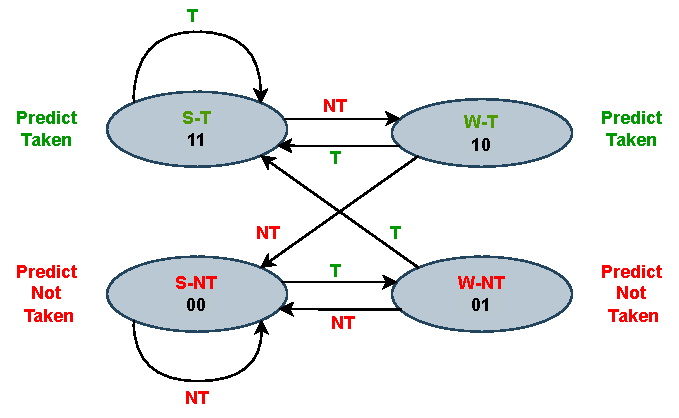
\includegraphics[width=0.75\linewidth]{alternate-fsm.pdf}
					\end{center}
				\end{figure}
				
				Ως μετρική χρησιμοποιούμε το direction Mispredictions Per Thousand Instructions (direction MPKI), στο οποίο θα αναφερόμαστε ως MPKI από εδώ και στο εξής. Έτσι έχουμε:
				
				\subsubsection{403.gcc}
					\begin{figure}[H]
						\begin{center}
							 \includegraphics[width=\myWidth]{\imagesPath/\dirba/\gcc}
						\end{center}
					\end{figure}

				\subsubsection{429.mcf}
					\begin{figure}[H]
						\begin{center}
							 \includegraphics[width=\myWidth]{\imagesPath/\dirba/\mcf}
						\end{center}
					\end{figure}

				\subsubsection{434.zeusmp}
					\begin{figure}[H]
						\begin{center}
							 \includegraphics[width=\myWidth]{\imagesPath/\dirba/\zeusmp}
						\end{center}
					\end{figure}

				\subsubsection{436.cactusADM}
					\begin{figure}[H]
						\begin{center}
							 \includegraphics[width=\myWidth]{\imagesPath/\dirba/\cactus}
						\end{center}
					\end{figure}

				\subsubsection{445.gobmk}
					\begin{figure}[H]
						\begin{center}
							 \includegraphics[width=\myWidth]{\imagesPath/\dirba/\gobmk}
						\end{center}
					\end{figure}

				\subsubsection{450.soplex}
					\begin{figure}[H]
						\begin{center}
							 \includegraphics[width=\myWidth]{\imagesPath/\dirba/\soplex}
						\end{center}
					\end{figure}

				\subsubsection{456.hmmer}
					\begin{figure}[H]
						\begin{center}
							 \includegraphics[width=\myWidth]{\imagesPath/\dirba/\hmmer}
						\end{center}
					\end{figure}

				\subsubsection{458.sjeng}
					\begin{figure}[H]
						\begin{center}
							 \includegraphics[width=\myWidth]{\imagesPath/\dirba/\sjeng}
						\end{center}
					\end{figure}

				\subsubsection{459.GemsFDTD}
					\begin{figure}[H]
						\begin{center}
							 \includegraphics[width=\myWidth]{\imagesPath/\dirba/\gems}
						\end{center}
					\end{figure}

				\subsubsection{462.libquantum}
					\begin{figure}[H]
						\begin{center}
							 \includegraphics[width=\myWidth]{\imagesPath/\dirba/\quantum}
						\end{center}
					\end{figure}

				\subsubsection{470.lbm}
					\begin{figure}[H]
						\begin{center}
							 \includegraphics[width=\myWidth]{\imagesPath/\dirba/\lbm}
						\end{center}
					\end{figure}

				\subsubsection{471.omnetpp}
					\begin{figure}[H]
						\begin{center}
							 \includegraphics[width=\myWidth]{\imagesPath/\dirba/\omnet}
						\end{center}
					\end{figure}

				\subsubsection{473.astar}
					\begin{figure}[H]
						\begin{center}
							 \includegraphics[width=\myWidth]{\imagesPath/\dirba/\astar}
						\end{center}
					\end{figure}

				\subsubsection{483.xalancbmk}
					\begin{figure}[H]
						\begin{center}
							 \includegraphics[width=\myWidth]{\imagesPath/\dirba/\xalanc}
						\end{center}
					\end{figure} 
				
				
				\subsubsection{Γεωμετρικός μέσος των benchmarks}
				
					Για λόγους συνολικής εποπτείας, παρουσιάζουμε και τον γεωμετρικό μέσο των benchmarks:
				
					\begin{figure}[H]
						\begin{center}
							\includegraphics[width=\myWidth]{\imagesPath/\dirba/gmean.pdf}
						\end{center}
					\end{figure}
			
				\subsubsection{Παρατηρήσεις}
					Παρατηρούμε ότι σε όλα τα benchmarks εκτός από τα \verb|434.zeusmp| και \verb|470.lbm|, η αύξηση των bits του predictor βελτιώνει τις επιδόσεις (μειώνεται το MPKI). Εξαίρεση αποτελεί η αύξηση από 3 bits σε 4 bits, η οποία δεν είναι πάντα βελτιωτική. Αξίζει να παρατηρηθεί βέβαια ότι στα benchmarks \verb|434.zeusmp| και \verb|470.lbm|, το MPKI είναι της τάξης του 0-2, οπότε οι διακυμάνσεις στις τιμές για διαφορετικές τιμές του $N$ είναι σχεδόν αμελητέες. \\
					
					Όσον αφορά το εναλλακτικό FSM που υλοποιήθηκε, αυτό δεν αποδίδει ποτέ καλύτερα από τον αντίστοιχο 2-bit predictor (saturating up-down counter) που υπήρχε στον βοηθητικό κώδικα που μας δόθηκε. \\
					
					Σύμφωνα με τον γεωμετρικό μέσο όρο των benchmarks, ο οποίος συμφωνεί με τα παραπάνω συμπεράσματα, ο καλύτερος predictor είναι ο \textbf{Nbit-16K-3bit}.
				
			\subsubsection*{(ii)}
				 Αυτή τη φορά διατηρούμε σταθερό το hardware (ίσο με $32\text{K}=2^{15}$ bits), ενώ το $N$ παίρνει πάλι τιμές $\{1,2,3,4\}$. Επομένως θα έχουμε:
				 
				 \begin{itemize}
				 	\item $\text{BHT entries}=32\text{K}$ και $N=1$
				 	\item $\text{BHT entries}=16\text{K}$ και $N=2$
				 	\item $\text{BHT entries}=16\text{K}$ και $N=2\text{β}$ (εναλλακτικό FSM)
				 	\item $\text{BHT entries}=8\text{K}$ και $Ν=4$
				 \end{itemize}
			 
			 	Έχουμε:
			 	
				\subsubsection{403.gcc}
					\begin{figure}[H]
						\begin{center}
							 \includegraphics[width=\myWidth]{\imagesPath/\dirbb/\gcc}
						\end{center}
					\end{figure}
				
				\subsubsection{429.mcf}
					\begin{figure}[H]
						\begin{center}
							 \includegraphics[width=\myWidth]{\imagesPath/\dirbb/\mcf}
						\end{center}
					\end{figure}
				
				\subsubsection{434.zeusmp}
					\begin{figure}[H]
						\begin{center}
							 \includegraphics[width=\myWidth]{\imagesPath/\dirbb/\zeusmp}
						\end{center}
					\end{figure}
				
				\subsubsection{436.cactusADM}
					\begin{figure}[H]
						\begin{center}
							 \includegraphics[width=\myWidth]{\imagesPath/\dirbb/\cactus}
						\end{center}
					\end{figure}
				
				\subsubsection{445.gobmk}
					\begin{figure}[H]
						\begin{center}
							 \includegraphics[width=\myWidth]{\imagesPath/\dirbb/\gobmk}
						\end{center}
					\end{figure}
				
				\subsubsection{450.soplex}
					\begin{figure}[H]
						\begin{center}
							 \includegraphics[width=\myWidth]{\imagesPath/\dirbb/\soplex}
						\end{center}
					\end{figure}
				
				\subsubsection{456.hmmer}
					\begin{figure}[H]
						\begin{center}
							 \includegraphics[width=\myWidth]{\imagesPath/\dirbb/\hmmer}
						\end{center}
					\end{figure}
				
				\subsubsection{458.sjeng}
					\begin{figure}[H]
						\begin{center}
							 \includegraphics[width=\myWidth]{\imagesPath/\dirbb/\sjeng}
						\end{center}
					\end{figure}
				
				\subsubsection{459.GemsFDTD}
					\begin{figure}[H]
						\begin{center}
							 \includegraphics[width=\myWidth]{\imagesPath/\dirbb/\gems}
						\end{center}
					\end{figure}
				
				\subsubsection{462.libquantum}
					\begin{figure}[H]
						\begin{center}
							 \includegraphics[width=\myWidth]{\imagesPath/\dirbb/\quantum}
						\end{center}
					\end{figure}
				
				\subsubsection{470.lbm}
					\begin{figure}[H]
						\begin{center}
							 \includegraphics[width=\myWidth]{\imagesPath/\dirbb/\lbm}
						\end{center}
					\end{figure}
				
				\subsubsection{471.omnetpp}
					\begin{figure}[H]
						\begin{center}
							 \includegraphics[width=\myWidth]{\imagesPath/\dirbb/\omnet}
						\end{center}
					\end{figure}
				
				\subsubsection{473.astar}
					\begin{figure}[H]
						\begin{center}
							 \includegraphics[width=\myWidth]{\imagesPath/\dirbb/\astar}
						\end{center}
					\end{figure}
				
				\subsubsection{483.xalancbmk}
					\begin{figure}[H]
						\begin{center}
							 \includegraphics[width=\myWidth]{\imagesPath/\dirbb/\xalanc}
						\end{center}
					\end{figure}
				
				\subsubsection{Γεωμετρικός μέσος των benchmarks} 
				
				\begin{figure}[H]
					\begin{center}
						\includegraphics[width=\myWidth]{\imagesPath/\dirbb/gmean.pdf}
					\end{center}
				\end{figure}
			
				\subsubsection{Παρατηρήσεις}
					Τα αποτελέσματα είναι ανάλογα με αυτά του προηγούμενου ερωτήματος. Εδώ με βάση τα διαγράμματα για κάθε benchmark αλλά και τον γεωμετρικό μέσο των αποτελεσμάτων, θα επιλέγαμε τον \textbf{Nbit-16K-2bit} predictor.
				
		\subsection{Μελέτη του BTB}
			Υλοποιούμε έναν BTB και μελετούμε την ακρίβεια πρόβλεψής του για τις περιπτώσεις:
			
			\begin{center}
				\begin{tabular}{|c|c|}
					\hline
					\textbf{BTB entries} & \textbf{BTB associativity} \\ \hline
					512 & 1 \\ \hline
					512 & 2 \\ \hline
					256 & 2 \\ \hline
					256 & 4 \\ \hline
					128 & 2 \\ \hline
					128 & 4 \\ \hline
					64  & 4 \\ \hline
					64  & 8 \\ \hline
				\end{tabular}
			\end{center}
			
			Έχουμε:
			
			\subsubsection{403.gcc}
				\begin{figure}[H]
					\begin{center}
						 \includegraphics[width=\myWidth]{\imagesPath/\dirc/\gcc}
					\end{center}
				\end{figure}
			
			\subsubsection{429.mcf}
				\begin{figure}[H]
					\begin{center}
						 \includegraphics[width=\myWidth]{\imagesPath/\dirc/\mcf}
					\end{center}
				\end{figure}
			
			\subsubsection{434.zeusmp}
				\begin{figure}[H]
					\begin{center}
						 \includegraphics[width=\myWidth]{\imagesPath/\dirc/\zeusmp}
					\end{center}
				\end{figure}
			
			\subsubsection{436.cactusADM}
				\begin{figure}[H]
					\begin{center}
						 \includegraphics[width=\myWidth]{\imagesPath/\dirc/\cactus}
					\end{center}
				\end{figure}
			
			\subsubsection{445.gobmk}
				\begin{figure}[H]
					\begin{center}
						 \includegraphics[width=\myWidth]{\imagesPath/\dirc/\gobmk}
					\end{center}
				\end{figure}
			
			\subsubsection{450.soplex}
				\begin{figure}[H]
					\begin{center}
						 \includegraphics[width=\myWidth]{\imagesPath/\dirc/\soplex}
					\end{center}
				\end{figure}
			
			\subsubsection{456.hmmer}
				\begin{figure}[H]
					\begin{center}
						 \includegraphics[width=\myWidth]{\imagesPath/\dirc/\hmmer}
					\end{center}
				\end{figure}
			
			\subsubsection{458.sjeng}
				\begin{figure}[H]
					\begin{center}
						 \includegraphics[width=\myWidth]{\imagesPath/\dirc/\sjeng}
					\end{center}
				\end{figure}
			
			\subsubsection{459.GemsFDTD}
				\begin{figure}[H]
					\begin{center}
						 \includegraphics[width=\myWidth]{\imagesPath/\dirc/\gems}
					\end{center}
				\end{figure}
			
			\subsubsection{462.libquantum}
				\begin{figure}[H]
					\begin{center}
						 \includegraphics[width=\myWidth]{\imagesPath/\dirc/\quantum}
					\end{center}
				\end{figure}
			
			\subsubsection{470.lbm}
				\begin{figure}[H]
					\begin{center}
						 \includegraphics[width=\myWidth]{\imagesPath/\dirc/\lbm}
					\end{center}
				\end{figure}
			
			\subsubsection{471.omnetpp}
				\begin{figure}[H]
					\begin{center}
						 \includegraphics[width=\myWidth]{\imagesPath/\dirc/\omnet}
					\end{center}
				\end{figure}
			
			\subsubsection{473.astar}
				\begin{figure}[H]
					\begin{center}
						 \includegraphics[width=\myWidth]{\imagesPath/\dirc/\astar}
					\end{center}
				\end{figure}
			
			\subsubsection{483.xalancbmk}
				\begin{figure}[H]
					\begin{center}
						 \includegraphics[width=\myWidth]{\imagesPath/\dirc/\xalanc}
					\end{center}
				\end{figure}
			
			\subsubsection{Γεωμετρικός μέσος των benchmarks}
			
				\begin{figure}[H]
					\begin{center}
						\includegraphics[width=\myWidth]{\imagesPath/\dirc/gmean.pdf}
					\end{center}
				\end{figure}
				
			\subsubsection{Παρατηρήσεις}
				Σημειώνεται ότι επειδή έχουμε να κάνουμε με BTB, υπάρχουν δύο περιπτώσεις misses, τα direction misprediction misses και τα target misprediction misses. \\
				
				Από τα διαγράμματα παρατηρούμε ότι για σταθερό πλήθος entries (γινόμενο ${\text{table lines} \times \text{associativity}}$ σταθερό), το associativity δρα βελτιωτικά. Συγκεκριμένα, για γινόμενο 512, ο BTB-64-8 έχει το μικρότερο MPKI, ενώ για γινόμενο 256, ο BTB-64-4 έχει τις καλύτερες επιδόσεις. Συνολικά, ο BTB-256-4 έχει συνολικά την καλύτερη επίδοση. Να σημειωθεί ότι ενώ σε κάποια benchmarks το MPKI φαίνεται να είναι σχεδόν 0, αυτό μπορεί να οφείλεται στο ότι τα συγκεκριμένα benchmarks δεν έχουν πολλές εντολές άλματος εξαρχής. Με βάση το διάγραμμα των γεωμετρικών μέσων, καλύτερη επίδοση φαίνεται να έχει ο \textbf{BTB-256-2} predictor.
				
		
		\subsection{Μελέτη του RAS}
			Σε αυτό το σημείο χρησιμοποιούμε το αρχείο \verb|ras.h|, το οποίο περιέχει μια υλοποίηση της RAS. Μελετούμε το ποσοστό αστοχίας για τις ακόλουθες περιπτώσεις:
			
			\begin{center}
				\begin{tabular}{|c|}
					\hline
					\textbf{Αριθμός εγγραφών στη RAS} \\ \hline
					4 \\ \hline
					8 \\ \hline
					16 \\ \hline
					32 \\ \hline
					48 \\ \hline
					64 \\ \hline
				\end{tabular}
			\end{center}
		
			Έχουμε:
			
			\subsubsection{403.gcc}
				\begin{figure}[H]
					\begin{center}
						 \includegraphics[width=\myWidth]{\imagesPath/\dird/\gcc}
					\end{center}
				\end{figure}
			
			\subsubsection{429.mcf}
				\begin{figure}[H]
					\begin{center}
						 \includegraphics[width=\myWidth]{\imagesPath/\dird/\mcf}
					\end{center}
				\end{figure}
			
			\subsubsection{434.zeusmp}
				\begin{figure}[H]
					\begin{center}
						 \includegraphics[width=\myWidth]{\imagesPath/\dird/\zeusmp}
					\end{center}
				\end{figure}
			
			\subsubsection{436.cactusADM}
				\begin{figure}[H]
					\begin{center}
						 \includegraphics[width=\myWidth]{\imagesPath/\dird/\cactus}
					\end{center}
				\end{figure}
			
			\subsubsection{445.gobmk}
				\begin{figure}[H]
					\begin{center}
						 \includegraphics[width=\myWidth]{\imagesPath/\dird/\gobmk}
					\end{center}
				\end{figure}
			
			\subsubsection{450.soplex}
				\begin{figure}[H]
					\begin{center}
						 \includegraphics[width=\myWidth]{\imagesPath/\dird/\soplex}
					\end{center}
				\end{figure}
			
			\subsubsection{456.hmmer}
				\begin{figure}[H]
					\begin{center}
						 \includegraphics[width=\myWidth]{\imagesPath/\dird/\hmmer}
					\end{center}
				\end{figure}
			
			\subsubsection{458.sjeng}
				\begin{figure}[H]
					\begin{center}
						 \includegraphics[width=\myWidth]{\imagesPath/\dird/\sjeng}
					\end{center}
				\end{figure}
			
			\subsubsection{459.GemsFDTD}
				\begin{figure}[H]
					\begin{center}
						 \includegraphics[width=\myWidth]{\imagesPath/\dird/\gems}
					\end{center}
				\end{figure}
			
			\subsubsection{462.libquantum}
				\begin{figure}[H]
					\begin{center}
						 \includegraphics[width=\myWidth]{\imagesPath/\dird/\quantum}
					\end{center}
				\end{figure}
			
			\subsubsection{470.lbm}
				\begin{figure}[H]
					\begin{center}
						 \includegraphics[width=\myWidth]{\imagesPath/\dird/\lbm}
					\end{center}
				\end{figure}
			
			\subsubsection{471.omnetpp}
				\begin{figure}[H]
					\begin{center}
						 \includegraphics[width=\myWidth]{\imagesPath/\dird/\omnet}
					\end{center}
				\end{figure}
			
			\subsubsection{473.astar}
				\begin{figure}[H]
					\begin{center}
						 \includegraphics[width=\myWidth]{\imagesPath/\dird/\astar}
					\end{center}
				\end{figure}
			
			\subsubsection{483.xalancbmk}
				\begin{figure}[H]
					\begin{center}
						 \includegraphics[width=\myWidth]{\imagesPath/\dird/\xalanc}
					\end{center}
				\end{figure}
		
			\subsubsection{Γεωμετρικός μέσος των benchmarks} 
			
				\begin{figure}[H]
					\begin{center}
						\includegraphics[width=\myWidth]{\imagesPath/\dird/gmean.pdf}
					\end{center}
				\end{figure}
			
			\subsubsection{Παρατηρήσεις}
				Σε όλα τα benchmarks, για 4 entries παρατηρείται πολύ μεγαλύτερο MPKI σε σχέση με τις μετέτειτα τιμές. Με αύξηση των entries πάντα το MPKI μειώνεται. Στις περισσότερες περιπτώσεις, μετά από 8 entries, δεν υπάρχει ουσιαστική αλλαγή στις επιδόσεις, αφού το MPKI έχει ουσιαστικά εκμηδενιστεί. Το γεγονός αυτό επηρεάζει και την επιλογή του βέλτιστου αριθμού entries, αφού θέλουμε να έχουμε τις καλύτερες επιδόσεις, με το ελάχιστο δυνατό υλικό. Επομένως, αφού από 16 entries και έπειτα έχει γίνει ήδη πολύ καλή βελτίωση της επίδοσης, επιλέγουμε αριθμό entries ίσο με \textbf{16}, και δεν κάνουμε overengineering στην RAS.
			
		
		\subsection{Σύγκριση διαφορετικών predictors}
			Σε αυτό το κομμάτι θα συγκρίνουμε τους παρακάτω predictors (όσοι είναι με \textbf{bold} δεν δίνονται και πρέπει να υλοποιηθούν)
			
			\begin{enumerate}
				\item \textbf{Static AlwaysTaken}
			
				\item \textbf{Static BTFNT (BackwardTaken-ForwardNotTaken)} 
			
				\item Ο N-bit predictor που επιλέξαμε στο 4.2 (ii). \\
				\textbf{Σημείωση:} Λόγω λάθους κατά την εκτέλεση του ερωτήματος  4.2 (ii), αρχικά φάνηκε ότι ο Nbit-8K-4bit predictor απέδιδε καλύτερα, οπότε επιλέξαμε αυτόν για το παρόν ερώτημα. Τελικά δεν έφτασε ο χρόνος για να ξαναεκτελεστούν τα benchmarks και να διορθωθεί το λάθος, οπότε στα παρακάτω διαγράμματα θα φαίνεται ο \textbf{Nbit-8K-4bit}.
			
				\item Pentium-M predictor (hardware overhead: $\approx$30K)
			
				\item \textbf{Local-History two-level predictor \#1} με τα εξής χαρακτηριστικά:
					\begin{itemize}
						\item PHT entries = 8K
						\item PHT N-bit counter length = 2
						\item BHT entries = 4K
						\item BHT entry length = 4 (ώστε το απαιτούμενο hardware να είναι ίσο με 32K)
					\end{itemize}
			
				\item \textbf{Local-History two-level predictor \#2} με τα εξής χαρακτηριστικά:
					\begin{itemize}
						\item PHT entries = 8K
						\item PHT N-bit counter length = 2
						\item BHT entries = 8K
						\item BHT entry length = 2 (ώστε το απαιτούμενο hardware να είναι ίσο με 32K)
					\end{itemize}
			
				\item \textbf{Global History two-level predictor \#1} με τα εξής χαρακτηριστικά:
					\begin{itemize}
						\item PHT entries = 8K (ώστε το απαιτούμενο hardware να είναι ίσο με 32K)
						\item PHT N-bit counter length = 2
						\item BHR length = 4
					\end{itemize}
			
				\item \textbf{Global History two-level predictor \#2} με τα εξής χαρακτηριστικά:
				\begin{itemize}
					\item PHT entries = 16K (ώστε το απαιτούμενο hardware να είναι ίσο με 32K)
					\item PHT N-bit counter length = 2
					\item BHR length = 8
				\end{itemize}
			
				\item \textbf{Global History two-level predictor \#3} με τα εξής χαρακτηριστικά:
				\begin{itemize}
					\item PHT entries = 8K (ώστε το απαιτούμενο hardware να είναι ίσο με 32K)
					\item PHT N-bit counter length = 4
					\item BHR length = 4
				\end{itemize}
			
				\item \textbf{Global History two-level predictor \#4} με τα εξής χαρακτηριστικά:
				\begin{itemize}
					\item PHT entries = 8K (ώστε το απαιτούμενο hardware να είναι ίσο με 32K)
					\item PHT N-bit counter length = 4
					\item BHR length = 8
				\end{itemize}
				
				\item \textbf{Alpha 21264 predictor} (hardware overhead: $\approx$29K)
				
				\item \textbf{Tournament Hybrid predictor \#1} με τα εξής χαρακτηριστικά:
					\begin{itemize}
						\item Ο meta-predictor $M$ είναι ένας 2-bit predictor με 1024 entries
						\item Ο $P_0$ είναι ένας \textbf{N-bit predictor} με τα εξής χαρακτηριστικά:
							\begin{itemize}
								\item BHT entries = 8K
								\item N = 2
							\end{itemize}
						\item Ο $P_1$ είναι επίσης ένας \textbf{N-bit predictor} με τα εξής χαρακτηριστικά:
							\begin{itemize}
								\item BHT entries =  4K
								\item N = 4
							\end{itemize}
						\item Οι $P_0, P_1$ έχουν overhead 16K ο καθένας
					\end{itemize}
				
				\item \textbf{Tournament Hybrid predictor \#2} με τα εξής χαρακτηριστικά:
					\begin{itemize}
						\item Ο meta-predictor $M$ είναι ένας 2-bit predictor με 2048 entries
						\item Ο $P_0$ είναι ένας \textbf{local-history predictor} με τα εξής χαρακτηριστικά:
							\begin{itemize}
								\item PHT entries = 4K
								\item PHT N-bit counter length = 2 bit
								\item BHT entries = 4K
								\item BHT entry length = 2 bit
							\end{itemize}
						\item Ο $P_1$ είναι ένας \textbf{N-bit predictor} με τα εξής χαρακτηριστικά:
							\begin{itemize}
								\item BHT entries = 8K 
								\item N = 2
							\end{itemize}
						\item Οι $P_0, P_1$ έχουν overhead 16K ο καθένας
					\end{itemize}
				
				\item \textbf{Tournament Hybrid predictor \#3} με τα εξής χαρακτηριστικά:
					\begin{itemize}
						\item Ο meta-predictor $M$ είναι ένας 2-bit predictor με 1024 entries
						\item Ο $P_0$ είναι ένας \textbf{global-history predictor} με τα εξής χαρακτηριστικά:
							\begin{itemize}
								\item PHT entries = 8K
								\item PHT N-bit counter length = 2
								\item BHR length = 8
							\end{itemize}
						\item Ο $P_1$ είναι ένας \textbf{N-bit predictor} με τα εξής χαρακτηριστικά:
							\begin{itemize}
								\item BHT entries = 4K 
								\item N = 4
							\end{itemize}
						\item Οι $P_0, P_1$ έχουν overhead 16K ο καθένας
					\end{itemize}
				
				\item \textbf{Tournament Hybrid predictor \#4} με τα εξής χαρακτηριστικά:
					\begin{itemize}
						\item Ο meta-predictor $M$ είναι ένας 2-bit predictor με 2048 entries
						\item Ο $P_0$ είναι ένας \textbf{local-history predictor} με τα εξής χαρακτηριστικά:
							\begin{itemize}
								\item PHT entries = 8K
								\item PHT N-bit counter length = 1
								\item BHT entries = 4K
								\item BHT entry length = 2
							\end{itemize}
						\item Ο $P_1$ είναι ένας \textbf{global-history predictor} με τα εξής χαρακτηριστικά:
							\begin{itemize}
								\item PHT entries = 4K
								\item PHT N-bit counter length = 4
								\item BHR length = 4
							\end{itemize}
						\item Οι $P_0, P_1$ έχουν overhead 16K ο καθένας
					\end{itemize}
			\end{enumerate}	
		
		Έχουμε:
		
		\subsubsection{403.gcc}
			\begin{figure}[H]
				\begin{center}
					 \includegraphics[width=\myWidth]{\imagesPath/\dire/\gcc}
				\end{center}
			\end{figure}
		
		\subsubsection{429.mcf}
			\begin{figure}[H]
				\begin{center}
					 \includegraphics[width=\myWidth]{\imagesPath/\dire/\mcf}
				\end{center}
			\end{figure}
		
		\subsubsection{434.zeusmp}
			\begin{figure}[H]
				\begin{center}
					 \includegraphics[width=\myWidth]{\imagesPath/\dire/\zeusmp}
				\end{center}
			\end{figure}
		
		\subsubsection{436.cactusADM}
			\begin{figure}[H]
				\begin{center}
					 \includegraphics[width=\myWidth]{\imagesPath/\dire/\cactus}
				\end{center}
			\end{figure}
		
		\subsubsection{445.gobmk}
			\begin{figure}[H]
				\begin{center}
					 \includegraphics[width=\myWidth]{\imagesPath/\dire/\gobmk}
				\end{center}
			\end{figure}
		
		\subsubsection{450.soplex}
			\begin{figure}[H]
				\begin{center}
					 \includegraphics[width=\myWidth]{\imagesPath/\dire/\soplex}
				\end{center}
			\end{figure}
		
		\subsubsection{456.hmmer}
			\begin{figure}[H]
				\begin{center}
					 \includegraphics[width=\myWidth]{\imagesPath/\dire/\hmmer}
				\end{center}
			\end{figure}
		
		\subsubsection{458.sjeng}
			\begin{figure}[H]
				\begin{center}
					 \includegraphics[width=\myWidth]{\imagesPath/\dire/\sjeng}
				\end{center}
			\end{figure}
		
		\subsubsection{459.GemsFDTD}
			\begin{figure}[H]
				\begin{center}
					 \includegraphics[width=\myWidth]{\imagesPath/\dire/\gems}
				\end{center}
			\end{figure}
		
		\subsubsection{462.libquantum}
			\begin{figure}[H]
				\begin{center}
					 \includegraphics[width=\myWidth]{\imagesPath/\dire/\quantum}
				\end{center}
			\end{figure}
		
		\subsubsection{470.lbm}
			\begin{figure}[H]
				\begin{center}
					 \includegraphics[width=\myWidth]{\imagesPath/\dire/\lbm}
				\end{center}
			\end{figure}
		
		\subsubsection{471.omnetpp}
			\begin{figure}[H]
				\begin{center}
					 \includegraphics[width=\myWidth]{\imagesPath/\dire/\omnet}
				\end{center}
			\end{figure}
		
		\subsubsection{473.astar}
			\begin{figure}[H]
				\begin{center}
					 \includegraphics[width=\myWidth]{\imagesPath/\dire/\astar}
				\end{center}
			\end{figure}
		
		\subsubsection{483.xalancbmk}
			\begin{figure}[H]
				\begin{center}
					 \includegraphics[width=\myWidth]{\imagesPath/\dire/\xalanc}
				\end{center}
			\end{figure}
		
		\subsubsection{Γεωμετρικός μέσος των benchmarks}
		
			\begin{figure}[H]
				\begin{center}
					\includegraphics[width=\myWidth]{\imagesPath/\dire/gmean.pdf}
				\end{center}
			\end{figure}
		
		\subsubsection{Παρατηρήσεις}
			Όπως είναι λογικό, ο Static AlwaysTaken predictor είναι ο χειρότερος από όλους, ενώ ακολουθεί ο Static BTFNT, καθώς αυτοί οι δύο predictors δεν διαθέτουν καθόλου "ευφυΐα". Ύστερα ακολουθεί ο Pentium-M predictor, ενώ οι υπόλοιποι predictors βρίσκονται περίπου στην ίδια τάξη επίδοσης (πχ 9-14\% στο \verb|403.gcc|). Σε όλα τα benchmarks η επίδοση του Alpha predictor είναι η καλύτερη, με εξαίρεση το \verb|445.gobmk|, όπου καλύτερος είναι ο Tournament predictor \#3 (όπως ορίστηκε παραπάνω). Αυτό έχει άμεση συνέπεια ο Alpha predictor να είναι ο καλύτερος και όσον αφορά τον γεωμετρικό μέσο όρο. Αυτό σημαίνει ότι πρόκειται και για την καλύτερη επιλογή, εκτός κι αν πραγματικά χρειαζόμαστε τις βέλτιστες επιδόσεις για μία πολύ συγκεκριμένη λειτουργία, η οποία μοιάζει πολύ με το \verb|445.gobmk|. Σε αυτή την περίπτωση, αξίζει να ελέγξουμε και τις επιλογές των Tournament \#3 και Global-History \#2. \\
	
			Τελικά, κατά μέσο όρο, η κατάταξη των predictors έχει ως εξής:
			
			\begin{verbatim}
				1.  Alpha 21264
				2.  Tournament #3
				3.  Global-History #2
				4.  Global-History #4
				5.  Local-History #1
				6.  Tournament #4
				7.  Global-History #3
				8.  Global-History #1
				9.  Local-History #2
				10. Tournament #2
				11. Tournament #1
				12. Nbit-8K-4
				13. Pentium-M
				14. Static BTFNT
				15. Static AlwaysTaken
			\end{verbatim}
	
\end{document}